\chapter{Requirements}
In this chapter, the requirements for a quantum-resistant variant of the MACSec protocol are discussed. For this reason, a scenario is described to define limitations that are derived from a real-world use-case. Both IEEE 802.1X and 802.1AE are designed for IEEE 802.3 Ethernet networks, which are available in various shapes. A limitation to common instances of such networks allows for a practically oriented design. For the same reason, a threat model that incorporates a realistic, albeit a futuristic example of a quantum computer that breaks common modern crypto schemes is required. To not weaken the design goals provided by the current design of MACSec, insight into the protocol suite is given to select currently used cryptographic guarantees and transfer them to the new design. Furthermore, it is important to identify currently used cryptographic primitives that are vulnerable to the definition of a general-purpose quantum computer and define requirements to solve these issues.

\section{Scenario}
IEEE 802.3 networks are usually deployed in the shape of either \acfp{LAN} or \acp{MAN}. \acp{LAN} usually include a full building or office space, with a few hundred to thousands of subscribers. Theoretically, the amount of devices in a single \ac{LAN} segment is not limited besides the possible address space of the used MAC addresses. However, in practice, a good approximation for a practical upper bound would be the size of a large office building with \(1,000\) to \(10,000\) devices. \acp{MAN} can be viewed as a special case of large \ac{LAN} installations, commonly used by large providers to provide internet access for small to medium-sized cities or districts in larger cities. While the number of subscribers can theoretically be even higher than in large office \ac{LAN} segments, the number of subscribers is expected to be in between a few orders of magnitudes. One example of a large \ac{MAN} installation is the \ac{MWN}, a large-scale network installation that connects research institutes, universities and student housing in Munich's metropolitan area. The \ac{MWN} uses about \(2,000\) switches to provide network connectivity to over \(100,000\) endpoints (Wireless and Wired)\cite{MWN}. For practical reasons, networks of this size are used as an upper bound in this work.

On the contrary, IEEE Ethernet networks can be relatively small. One example of networks with few subscribers and small amounts of computational capacities is \ac{IoT} networks, with nodes that are very limited in terms of memory and \acs{CPU} frequency when compared to a modern desktop computer. For example, the FIT IoT-LAB is a large-scale \ac{IoT} testbed used to run scientific experiments on real-world \ac{IoT} hardware. The hardware used in this testbed consists mostly of ARM Cortex M0-M4 \acp{MCU}, with processing frequencies ranging from multiple kilohertz to few megahertz and limited networking capabilities like IEEE 802.15.4	and LoRa\cite{adjih:hal-01213938}. The selection of requirements on a \ac{PQ} MACSec design should take both extremes into account and support networks with very few and limited nodes, as well as big networks with rather strong clients.


\section{Threat Model}
In the threat model used in this thesis, an attacker can perform attacks according to IND-CCA2. Furthermore, it is assumed that an attacker has access to a quantum computer that can break currently used state of the art asynchronous key exchanges, such as integer factorization-based methods, and methods based on the discrete logarithm problem in polynomial time. The used quantum computer should be able to perform Grover's algorithm to attack synchronous crypto schemes of arbitrary key sizes. It is further assumed that the attacker has access to a ``sufficiently large'' classical computer to perform brute force attacks on the used crypto scheme as well. In this context, it is safe to assume that ``sufficiently large'' means that an attacker has access to computing resources that match the size of so-called exascale systems, which can perform \(10^{18}\) \ac{FLOPS}.

\section{PQC Requirements}

In 802.1X and 802.1AE, both synchronous and asynchronous cryptographic schemes are used. For the initial key exchange, either a symmetric pre-shared key or an asymmetric key exchange is used. In both cases, symmetric schemes are used to derive further keys and ensure confidentiality. For both types of cryptosystems, requirements need to be defined to secure them against an attacker in possession of a quantum computer as described in the threat model. 

\subsection{Asynchronous Key Exchange}
To mitigate attacks that involve a quantum computer running Shor's algorithm, a quantum-resistant asynchronous crypto scheme needs to rely on alternative methods for asynchronous key exchanges than currently used. It is assumed that the ongoing \ac{NIST} standardization project candidates as described in Chapter~2 are secure against attacks that involve a quantum computer until proven otherwise. A design concerning the defined threat model also needs to consider that the discussed schemes may be vulnerable to not yet discovered attacks on classical computers. While the same argument holds for classical key exchange methods, the maturity of those systems provides confidence in the security of those cryptosystems.

For this reason, a quantum-resistant KEX mechanism should include a so-called hybrid scheme, which uses both a classical and a quantum-resistant scheme to provide resistance against an attack involving a quantum computer while providing a notion of forward-secrecy, even if the used post-quantum algorithm turns out to be weakened by an attack using either a classical or a quantum computer. While not supported directly in any \ac{NIST} standard, the \ac{NIST} provides recommendations on implementing such hybrid modes without losing compliance to \ac{FIPS} 140, a \ac{NIST} standard that defines security requirements on cryptographic systems. \ac{NIST} special publication 800-56C defines two methods for a key derivation function that can be used for this purpose\cite{barker2018recommendation}:

\begin{enumerate}
    \item \textbf{One-Step Key Derivation}\\
    For one-step \acp{KDF}, a hash, HMAC or KMAC one-way function is used to derive keying material. As an additional input to the one-way function, SP 800-56C allows for a \textit{FixedInfo} field as defined in SP 800-56A. The \textit{FixedInfo} field includes a \textit{SuppPrivInfo} parameter with additional arbitrary and mutually known private information that can be included in the key derivation. Alternatively, the key exchanged via a \ac{PQ} method can be included in the salt field.
    \item \textbf{Two-Step Key Derivation}\\ In the two-step method, the \ac{PQ} key can be included in the \ac{KDF} as a salt value for the HMAC or AES-CMAC expansion.
\end{enumerate}

For future versions of SP 800-56C, the \ac{NIST} plans to include the possibility for hybrid constructions in the standard directly. This can be done by allowing the input for both \acp{KDF} to be a concatenated value from two or more key exchange methods.\footurl{https://csrc.nist.gov/Projects/Post-Quantum-Cryptography/faqs}

\subsection{Comparison of NIST PQ-KEX Algorithms}
The algorithms in the current Round 3 of the \ac{NIST} \ac{PQ} project rely upon different mathematical foundations and depend on different cryptographic primitives. Therefore, all algorithms perform differently in terms of performance and provided security guarantees. Since a replacement for currently used cryptographic primitives in IEEE 802.1X and IEEE 802.1AE needs to take these differences into account, a short overview of the requirements is provided in this section. Further, a brief comparison of all Round 3 algorithms is shown. Common restrictions on asynchronous cryptographic key exchange protocols are the amount of additional traffic due to key and ciphertext sizes and the computational overhead to de- and encrypt a single key. When taking forward-secrecy into account, the key generation time is an additional important factor. For cryptographic protocols that do not provide a built-in forward-secrecy notion, this can only be achieved by generating a new key pair for each connection. The only protocol in the \ac{NIST} project that claims to provide the notion of forward-secrecy by design is SIKE.

\subsubsection{\acf{PFS}}

\begin{figure}[ht]
    \centering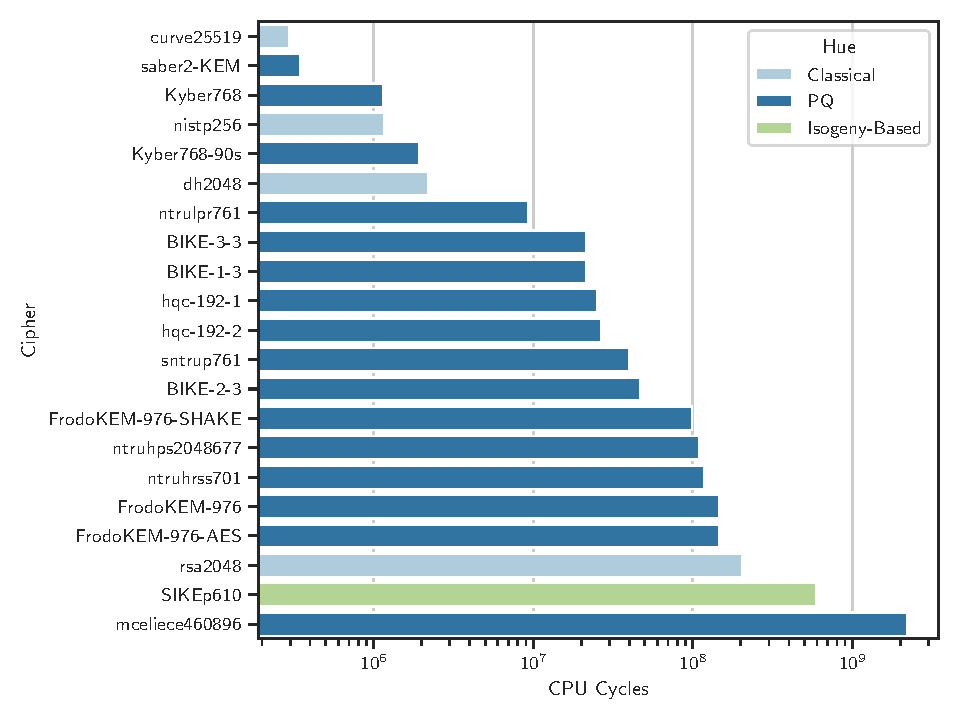
\includegraphics[width=0.9\linewidth]{plot_bar_ephemeral.pdf}
    \caption{CPU cycles for a single ephemeral key exchange on a logarithmic axis. In the case of \texttt{SIKE} and EC(DH)-based schemes, the time for the computation of a shared secret is shown. The remainder of the ciphers shows the combined time for the generation of a fresh key pair in addition to the time to compute a shared secret. Benchmark results are part of eBACS\cite{eBACS}. Only implementations concerning security level 3 are shown.}\label{fig:ephemeral}
\end{figure}

When \ac{EAP} is used for MACSec key agreement, a session key is generated via the appropriate \ac{EAP} method. A session key is used as seeding material for a pairwise \ac{CAK} between the Authenticator and the Supplicant. A group \ac{CAK} seeded by the pairwise \acp{CAK} can be further generated by the Authenticator for distribution to the clients. The group \ac{CAK} is used to agree on a shared key in a MACSec \ac{CA} and is distributed cryptographically secured by the pairwise \acp{CAK}. For this reason, the secret of the distributed \ac{CAK} relies on the secret of all pairwise \acp{CAK}. Using a cryptographic method for key exchange that allows for forward-secrecy would ensure that a subsequent group \ac{CAK} could not be derived from recorded key exchanges if the long-term key of the Authenticator is breached in any way and thus would be preferable for the key exchange method. For \ac{PQ} key exchange methods, SIKE is a natural candidate for a protocol that supports forward-secrecy. Alternatively, any \ac{KEX} method with a fresh key pair for each session can be used to achieve forward-secrecy. When taking into account that a key exchange in SIKE is relatively costly compared to alternative \ac{PQ} key exchange methods, it may be even faster to use this construction to achieve \ac{PFS} as opposed to using SIKE. Figure~\ref{fig:ephemeral} shows the cost of an ephemeral key exchange for all \ac{NIST} \ac{PQ} ciphers with a security level of 3. In the case of SIKE, only the time for encapsulation and decapsulation of a single key is shown. To get a comparable notion of forward-secrecy, the other candidates additionally show the time to generate a fresh key pair. As a baseline, the times for \texttt{RSA} using a 2048 bit key, for \ac{DH} with 2048 bit and two \ac{ECDH} schemes, using \texttt{curve25519} and \texttt{nistp256} are shown. The plot shows that using any other algorithm except \texttt{mceliece460896} with a fresh key pair for each session is more efficient in terms of computational costs than using SIKE with a single key while providing the same guarantees regarding forward-secrecy.

\subsubsection{Computational Overhead}

\begin{figure}[ht]
    \centering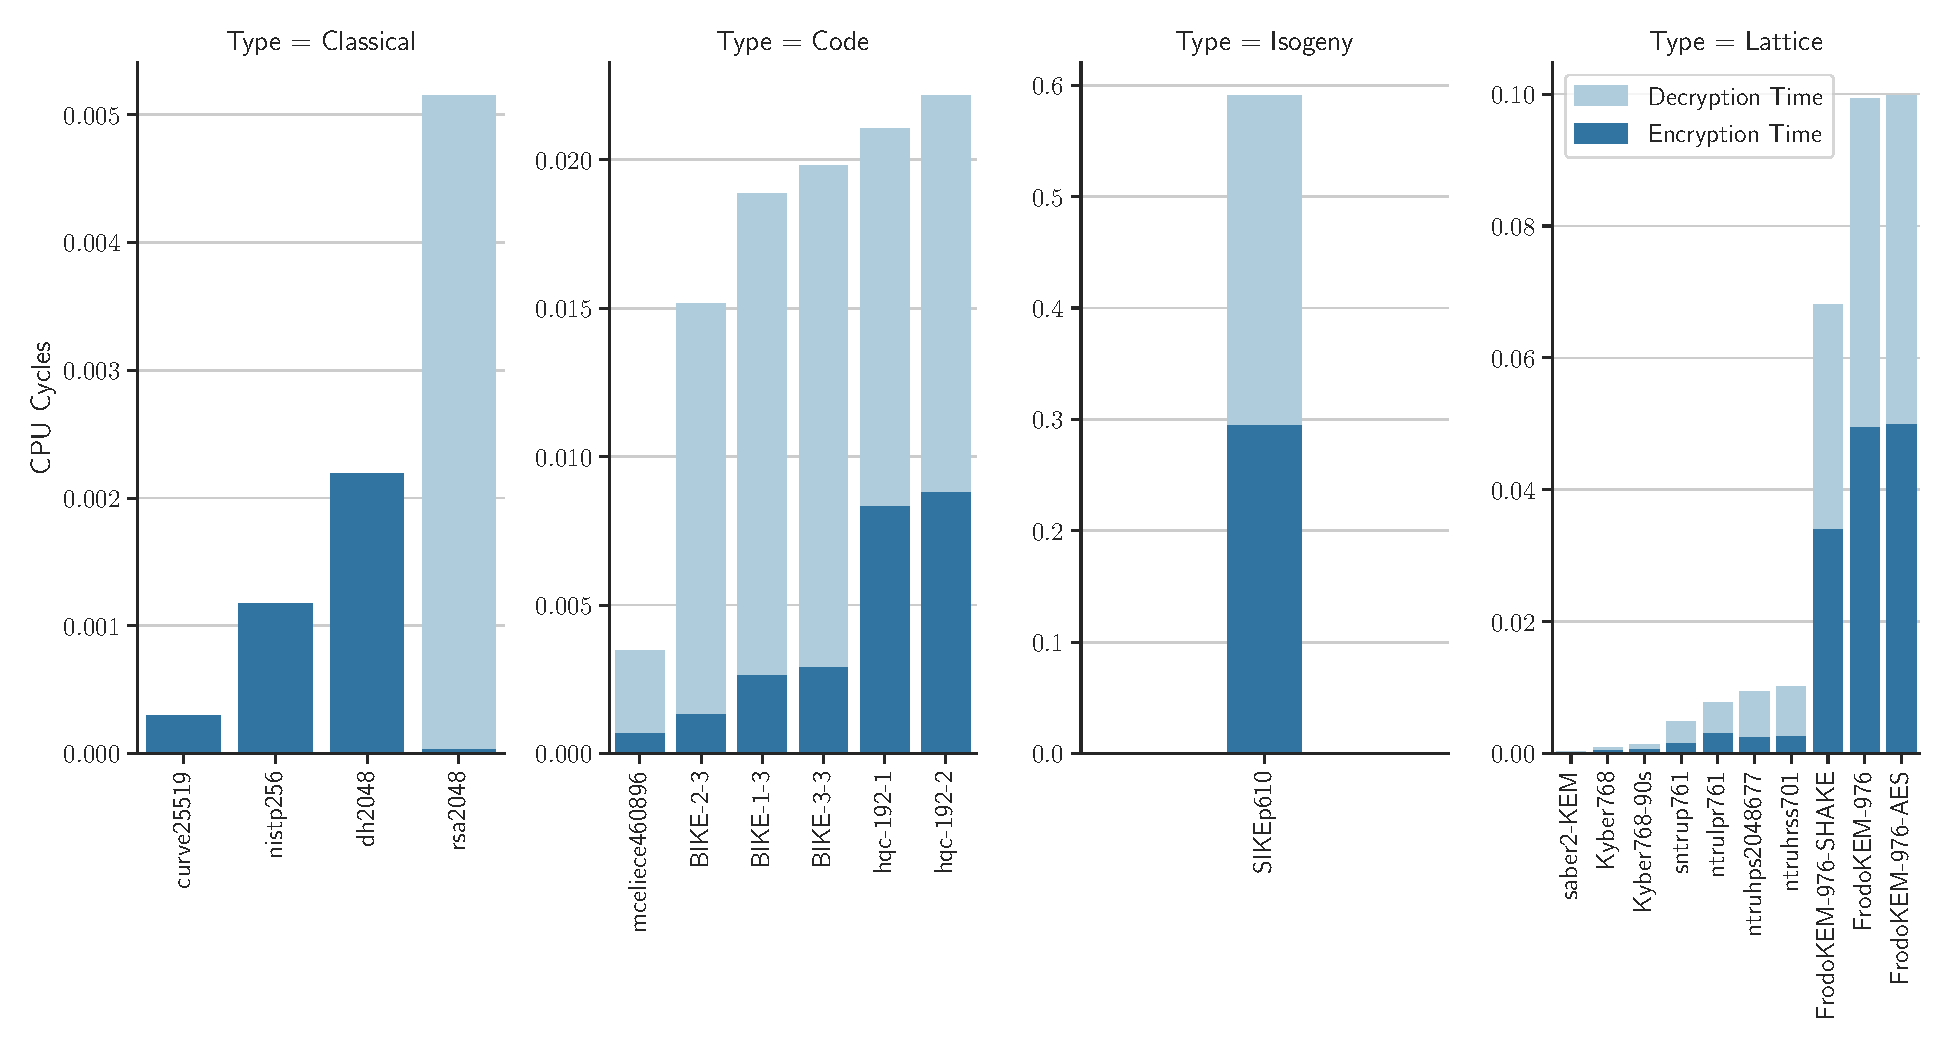
\includegraphics[width=1\linewidth]{plot_bar_enc_dec.pdf}
    \caption{The time needed to exchange a single shared secret in \(10^9\) \ac{CPU} cycles. Benchmark results are part of eBACS\cite{eBACS}. Only implementations concerning security level 3 are shown.}\label{fig:pq_computing}
\end{figure}

Another important metric for a key exchange protocol is the amount of computational overhead for a single key exchange. The amount of computing time spent on a single key exchange is the sum of the time for key encapsulation on one side and the time for key decapsulation on the other side. Additionally, the key generation time needs to be taken into account. The computational overhead is especially significant in scenarios like IEEE 802.1X, where the Authenticator can be some sort of special-purpose network equipment with rather slow general-purpose computing units, or in scenarios involving \ac{IoT} endpoints. For \ac{PQ} key exchange methods, the computational overhead strongly depends on the used type of algorithms. Figure~\ref{fig:pq_computing} shows an overview of time spent on a single encapsulation and decapsulation in \(10^9\) CPU cycles. It shows that code-based schemes perform well, with some lattice-based schemes as close competitors. SIKE performs worst due to a large amount of finite field arithmetic performed in each key exchange. More optimized implementations are available for some algorithms to reduce the cycle count by a large factor. For example, using an optimized assembly implementation for SIKEp751 reduces the cycle count for a single key exchange operation by a factor \(10\). Even better results can be achieved by using an FPGA-based implementation tailored to a certain algorithm implementation. The plot shows the fastest available implementation in eBACS. When no such implementation is available, the fastest available implementation provided by the authors is shown.

\subsubsection{Communication Overhead}

\begin{figure}[ht]
    \centering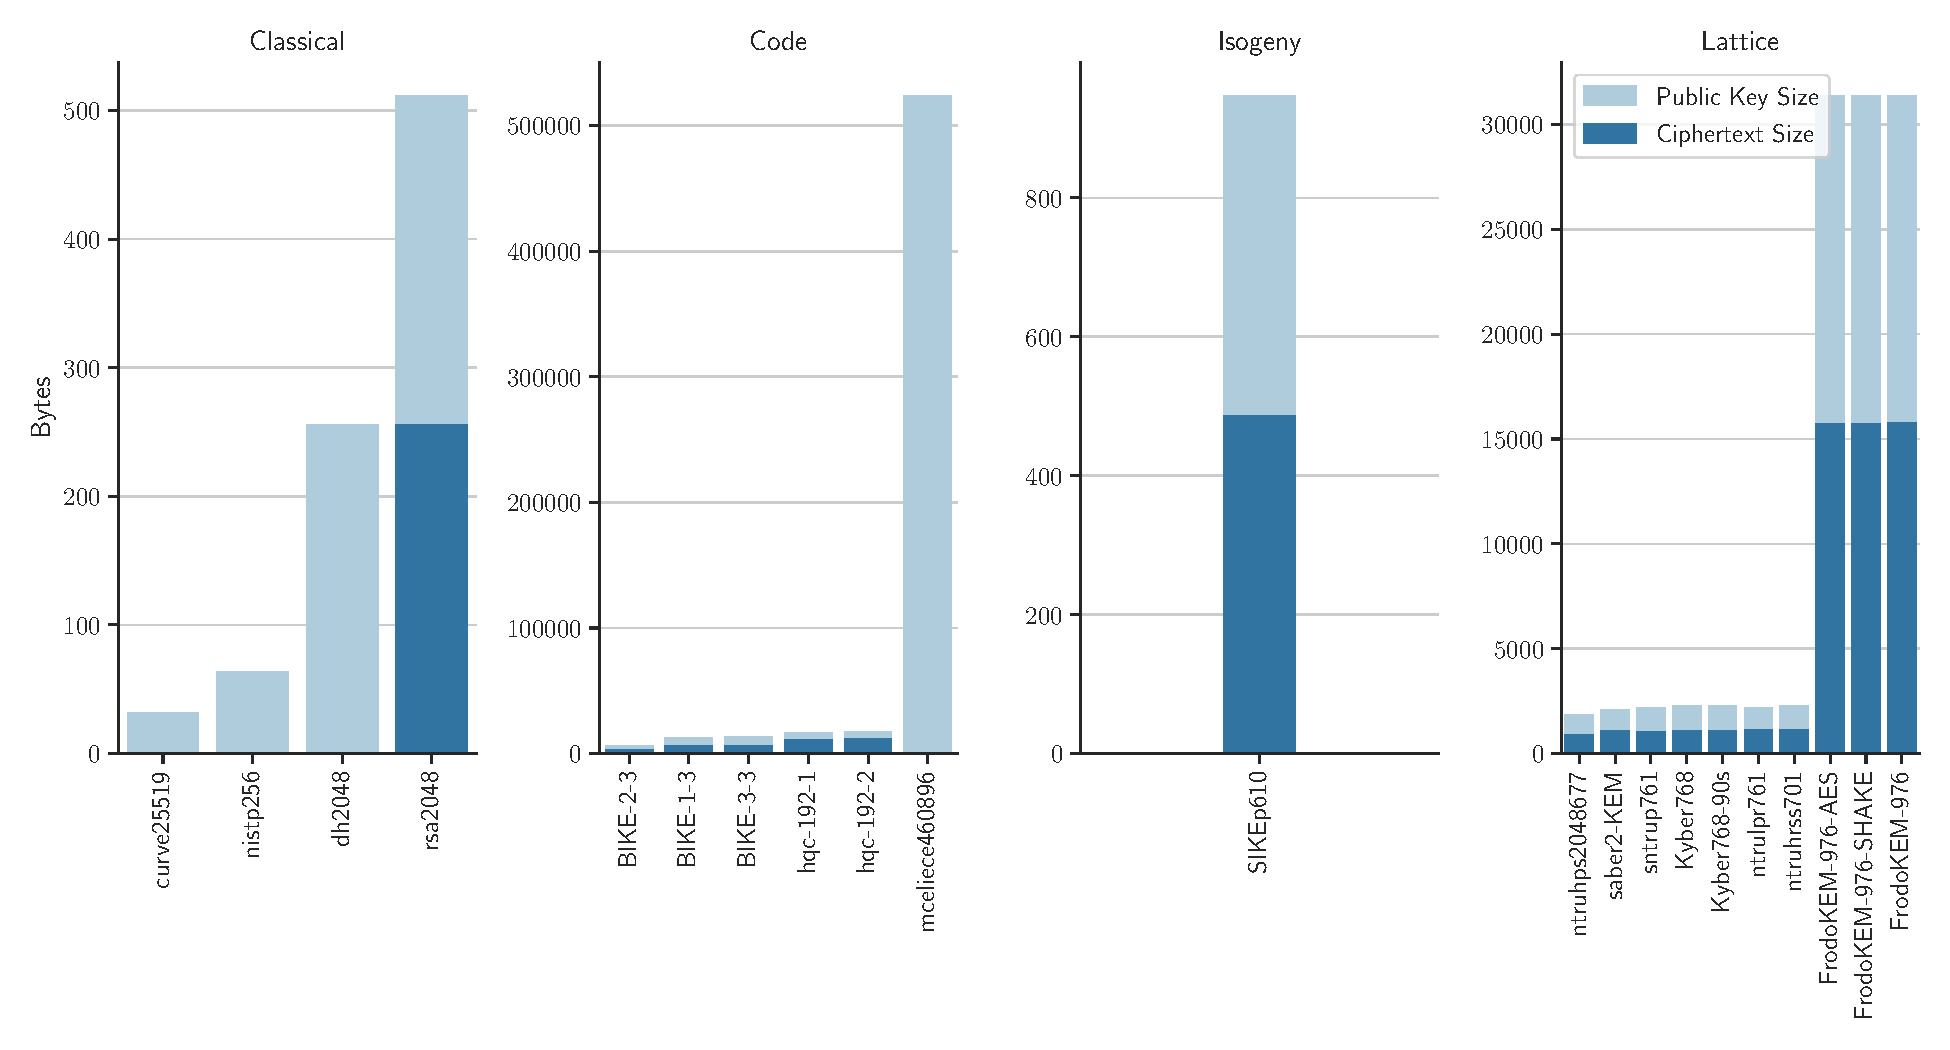
\includegraphics[width=1\linewidth]{plot_bar_traffic.pdf}
    \caption{Network communication in Bytes for a single key exchange. Benchmark results are part of eBACS\cite{eBACS}. Only implementations concerning security level 3 are shown.}\label{fig:pq_traffic}
\end{figure}

Another concern regarding the used \ac{PQ} key exchange method is the amount of generated traffic for a single key exchange. Assuming the public key is not cached or pre-transferred to the client, the traffic pattern of a full key exchange usually includes the public key and a shared secret of a certain size. The size of the public key may be decreased by a compression algorithm. The size of the ciphertext often is increased by some factor depending on the used cryptosystem. Code-based schemes, for example, need to transfer the cleartext into a codeword of a certain size by adding some redundant information. The exact blow-up factor is depending on the used primitives and the security level of the cipher. Reducing traffic is important for multiple reasons. First, a smaller communication footprint saves time when the throughput of the connection is a limiting factor.

Further, in cases where many key exchanges occur simultaneously, a smaller traffic pattern may decrease costs in the backbone since network links to Authentication Servers can be provisioned more conservatively. Another reason to decrease the communication size is the need to fit the key exchange in a few or even a single package for configurations where the size of a single packet is limited. For example, a single Ethernet frame is usually limited to a size of 1500 Bytes. For public keys or ciphertext messages that exceed this size, some sort of fragmentation is needed to ensure the frames can be fully transmitted. In the case of IEEE 802.1X, network traffic is not that much of a concern. Usually, the authentication takes place in \acp{LAN}, where either Ethernet or IEEE 802.11 wireless networks are used, which support bandwidths ranging from 100 MB/s to a few GB/s. Figure~\ref{fig:pq_traffic} shows the required communication cost in Bytes to transmit a single public key without compression and for a ciphertext that contains a shared secret of 32 Bytes. While the variance in the required size for a single key exchange is rather high, most of the displayed algorithms require less than a single KB of data. Even in the extreme case, the data size is below a single MB.

Additionally, 802.1X-secured channels are relatively long-lived. A client only needs to authenticate once it plans to join the network. While re-authentication is part of 802.1X, the proposed default value for the re-authentication time is set to once every 3200 seconds[Section~8.6]\cite{IEEE8021X}. Even if rather large networks with \(10.000\) subscribers are assumed, only a few megabyte traffic would be generated, assuming a rather large data size of 1 MB per authentication attempt. The traffic pattern can be further optimized by using multiple Authentication Servers and, therefore, keep the traffic in a local environment. Additionally, the authentication can be directly performed on the Authenticator without the need for an external Authentication Server. Regarding packet fragmentation, IEEE802.1X states that the used \ac{EAP} method should have built-in fragmentation support if it is needed by the method[Section~8.11.1]\cite{IEEE8021X}.

\subsubsection{Summary}

For the design of the cryptosystem, it is important to add additional security and not lose already available guarantees. Therefore, \ac{PFS} support should be available by the used key exchange method as the main concern. This can be either achieved by using an implementation that already supports this notion, like SIKE. Or using a fresh key pair for each session with any other key exchange algorithm. For the use case of constrained environments like network equipment or mobile and \ac{IoT} endpoints, the computational overhead of the implementation is the next important factor to consider. While the actual work can be performed by an external Authentication Server in the case of 802.1X, this is not necessarily true for all implementation and saving resources on these constrained devices may benefit the overall performance of the network. The last factor to consider is the amount of traffic a cryptosystem adds to the network. While the amount of additional traffic for the NIST Round 3 candidates may look significant when compared to light-weight DH-based protocols, it is often negligible in modern \ac{LAN} infrastructures. This is due to a large amount of bandwidth usually available and the low frequency of authentication operations in IEEE 802.1X when compared to high-frequency applications like web or email servers. Therefore the requirements on the used algorithm should be considered in the following order:

\begin{enumerate}[itemsep=0pt]
    \item \acl{PFS}
    \item Cycles for a single key exchange (Computation Overhead)
    \item Traffic for a single key exchange (Communication Overhead)
\end{enumerate}

\subsection{Asynchronous Signature Schemes}
Analogous to asynchronous key exchange methods, currently used signature schemes used for authentication are vulnerable to attacks under the given threat model. To solve this problem, a notion similar to hybrid modes called dual-signatures is commonly used. In such scenarios, a message is signed multiple times, either by a composition of two signatures or by sending two distinct signatures. Unlike for hybrid key exchange methods, the \ac{NIST} does not make any recommendations on how to accommodate dual signatures into existing standards and leaves this task up to the implementation. The \ac{NIST} states that the \ac{FIPS} compliance of the signature validation is given as long as one of the signature schemes is a properly implemented \ac{NIST} scheme according to \ac{FIPS} 140.

\subsection{Comparison of NIST PQ Signature Algorithms}

Unlike for \ac{PQ} key exchange mechanisms, leaking the long term key used for signature creation and validation has no retrospective security implication since the authenticity of a message is only relevant once a message is received. For this reason, the notion of \ac{PFS} does not apply. The two main considerations regarding \ac{PQ} signature schemes are the amount of additional traffic generated for a signature and the amount of computational overhead created on both sides for the creation and validation of the signature. 

\subsubsection{Computation Overhead}
\begin{figure}[ht]
    \centering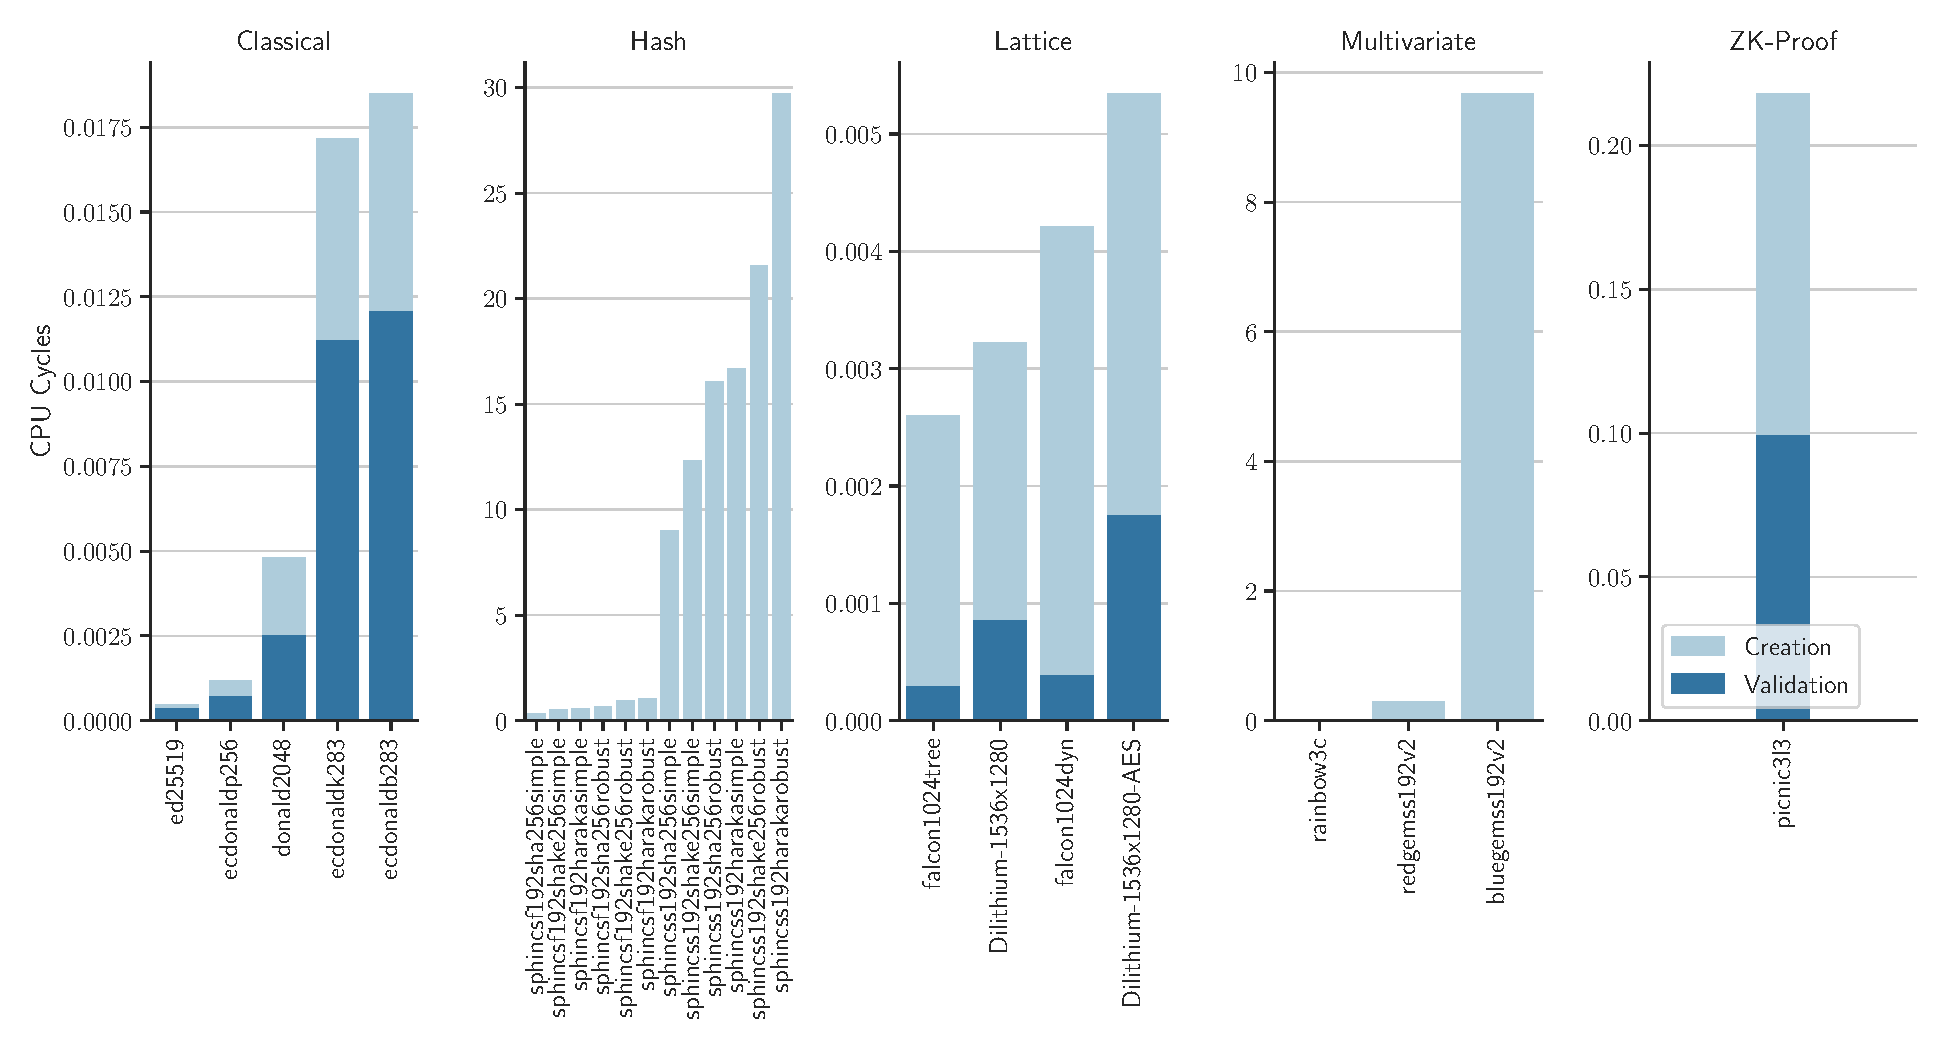
\includegraphics[width=1\linewidth]{plot_bar_comp_signature.pdf}
    \caption{Computational effort for the creation and validation of a single signature in \(10^9\) \acs{CPU} cycles. Benchmark results are part of eBACS\cite{eBACS}. Only implementations concerning security level 3 are shown.}\label{fig:pq_sig_comp}
\end{figure}

An authentication procedure involving digital signatures consists of the creation and validation of the signature. For most participants in the \ac{NIST} \ac{PQ} project, as shown in Figure~\ref{fig:pq_sig_comp}, the overhead for the signature creation is rather big compared to the overhead for validation and sometimes even dominates the workload entirely. In the case of IEEE 802.1X, both the Authenticator and the Peer need to create a valid signature for mutual authentication in every session. For this reason, the imbalance of the two tasks is not as important as the sum of the overall overhead for validation and creation of a single signature. Speaking in total numbers, lattice-based signatures perform rather fast in comparison to classical digital signature schemes, with \texttt{Picnic} as a close competitor. Multivariate signature schemes, with the exception of \texttt{redgemss}, also provide a reasonable value in comparison with other schemes. When using \texttt{SPHINCS+} as a hash-based signature, the computational overhead strongly depends on whether an ``\texttt{f}'' or an ``\texttt{s}'' implementation is used, with a significant performance advantage for the ``\texttt{f}''-variants.

\subsubsection{Communication Overhead}
\begin{figure}[ht]
    \centering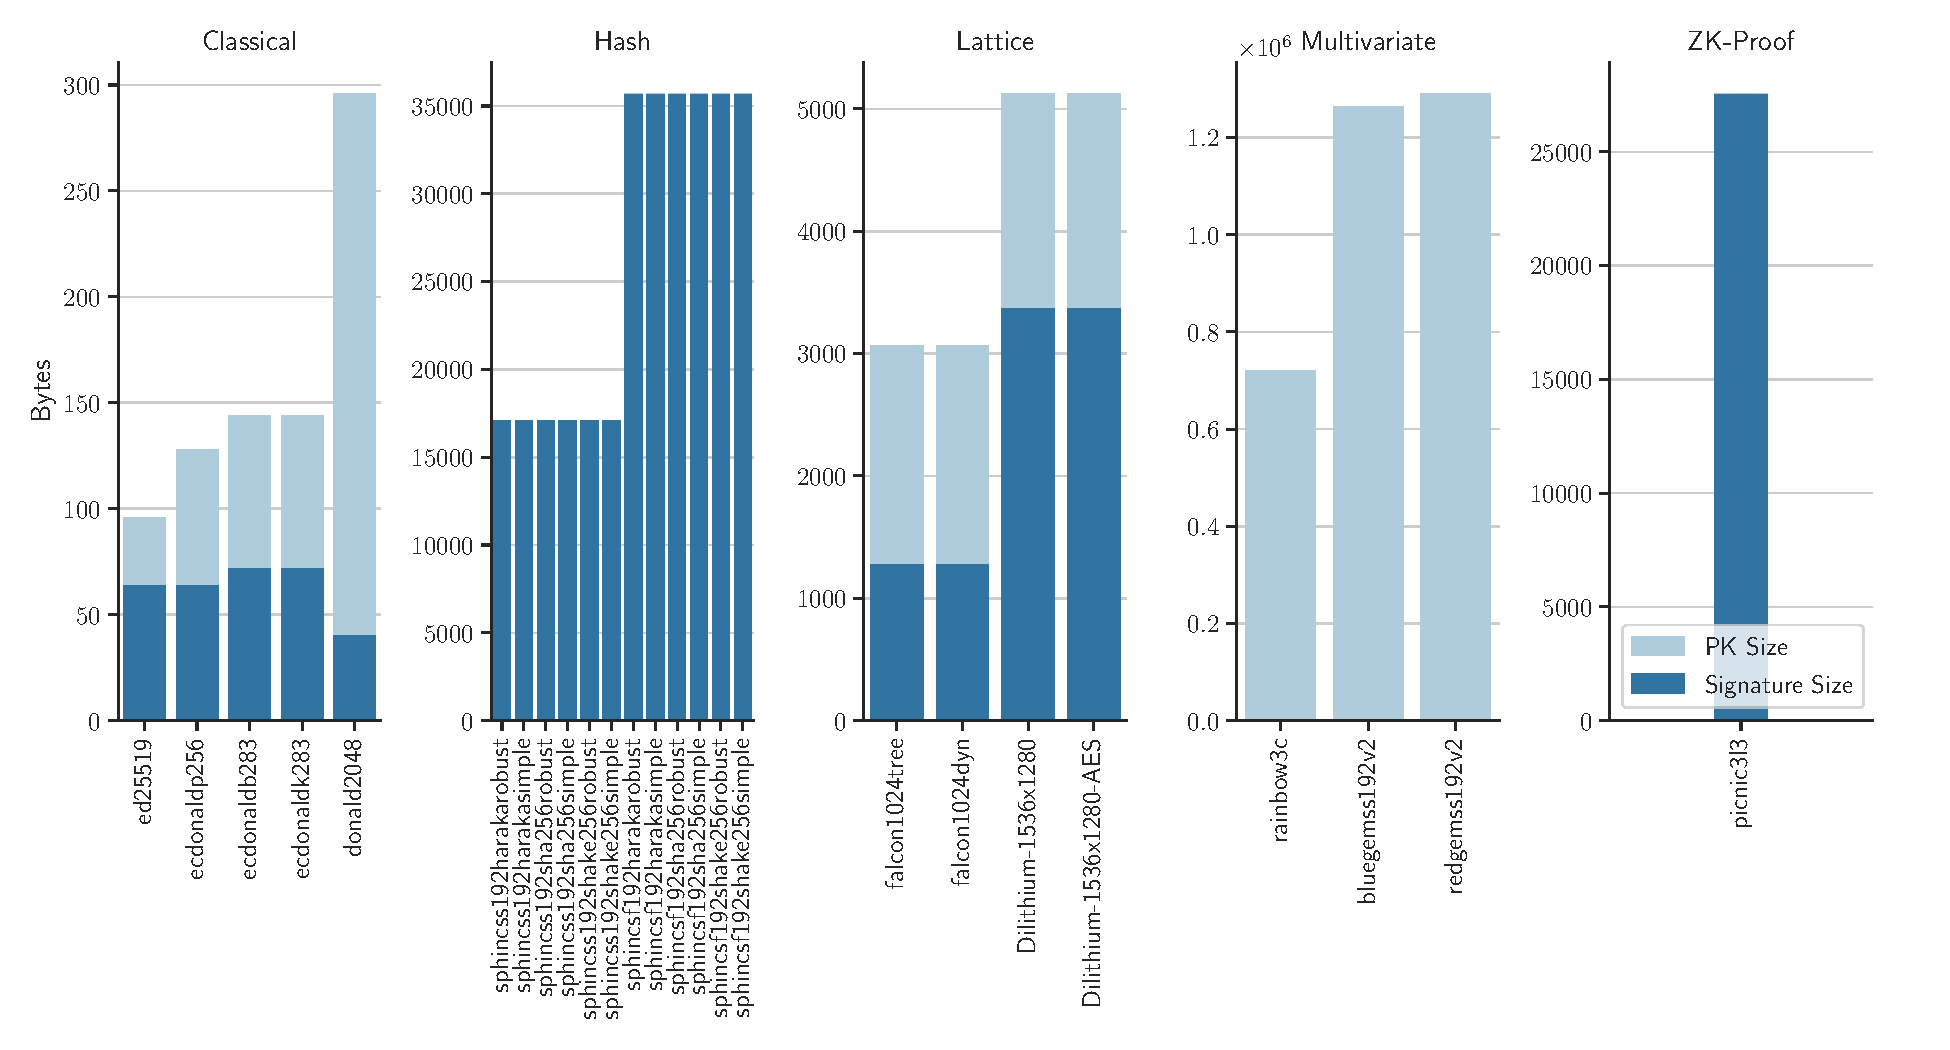
\includegraphics[width=1\linewidth]{plot_bar_traffic_signatures.pdf}
    \caption{Network communication in Bytes for one signature. Benchmark results are part of eBACS\cite{eBACS}. Only implementations concerning security level 3 are shown.}\label{fig:pq_sig_traffic}
\end{figure}

In terms of communication overhead, there is a large gap between \ac{PQ} algorithms and classical algorithms, which can be as large as a factor of \(10^4\) for multivariate signature schemes. Figure~\ref{fig:pq_sig_traffic} shows the amount of data in bytes that need to be transferred to perform a single signature, ranging from a few KB to a few MB. When only taking algorithms with security level 3 into account, the smallest available \ac{PQ} cipher already needs to transfer twenty to fifty times as much data as RSA- or \ac{DH}-based signature schemes. When considering the mutual authentication setting in 802.1X, the gap between classical approaches and \ac{PQ} algorithms gets even more relevant since public keys and signatures need to be transferred by each peer. Compared to classical signature schemes, lattice-based \ac{PQ} signatures show the smallest traffic overhead, with values ranging within a few KB of each other. In this case, the size of the signature and the size of the public keys contribute about the same amount to the overall traffic. Other interesting alternatives with a rather little traffic pattern are hash-based signatures, with signature sizes of \(15\) to \(40\) KB. Contrary to lattice-based signatures, the ratios of signature to public-key sizes in hash-based variants are rather extreme since the sizes of the public keys usually only are the size of a single hash-value with a few bytes. In the case of Picnic, the results are similar to hash-based variants. The overall traffic needed for a single authentication is almost entirely dominated by the signature sizes and needs about 30 KB for \texttt{picnic} with security level 3. The multivariate signatures shown in the plot are rather extreme when com+pared to the rest of the algorithms. While the signatures themselves only require a few bytes of traffic, the public keys have a size of around 1 MB. It is important to notice that public keys of certificate-chains can be cached by both participants while the signatures need to be created and transferred in every session. This emphasizes the value of using small signatures over using an algorithm with small public keys. It is important to keep in mind that at least the client-certificates need to be transferred for every authentication, and therefore a compromise needs to be found between signature and public key sizes.


\subsubsection{Summary}

\begin{figure}[ht]
    \centering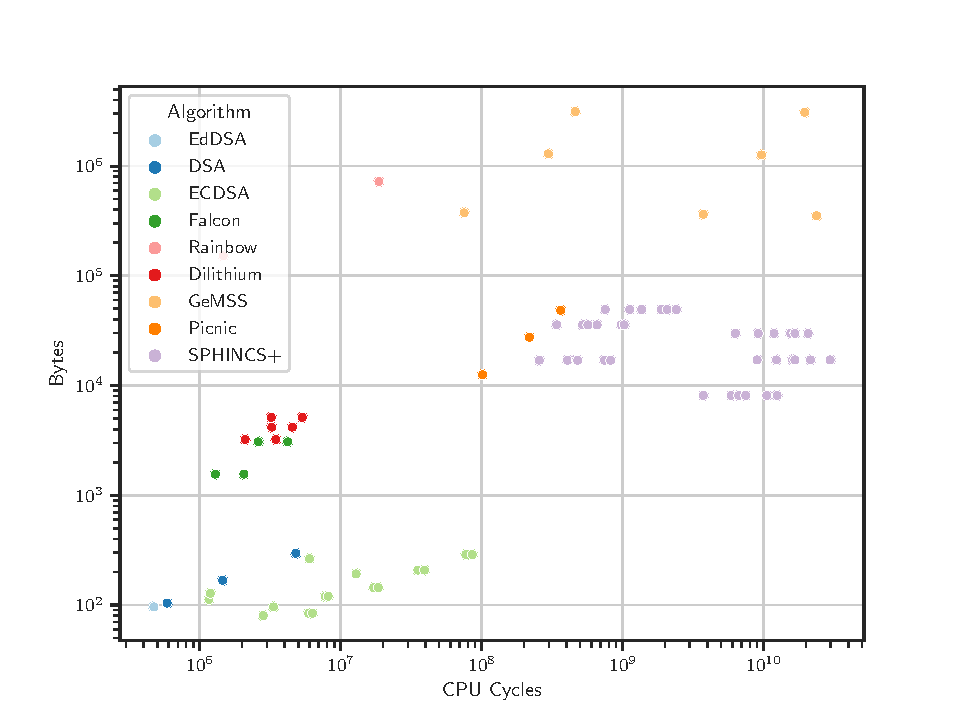
\includegraphics[width=1\linewidth]{plot_bar_cycles_bytes_signature.pdf}
    \caption{\acs{CPU} cycles and bytes traffic for one single signature creation and validation. Both axes are displayed on a logarithmic scale. Benchmark results are part of eBACS\cite{eBACS}.}\label{fig:pq_sig_c_b}
\end{figure}

When taking into account that some \ac{PQ} signature algorithms can compete with classical algorithms in terms of computational overhead but may introduce a large amount of data transfer on every authentication, the amount of transferred data becomes more of a concern than in the case for key exchange algorithms. Figure~\ref{fig:pq_sig_c_b} shows the values for both the number of \acs{CPU} cycles and the amount of data traffic for a single signature creation in comparison to other algorithms. While all \ac{PQ} algorithms introduce significant overhead in both variables, some ciphers can compete with their classical counterparts. Especially, Dilithium and Falcon (two lattice-based variants) show values close within one to two orders of magnitude with respect to the traffic size. When looking at the computational overhead, both algorithms even perform as good as or even better than some classical schemes.

\subsection{Synchronous Schemes}

\begin{table}[t]
    \centering
    \caption{Average time to find a key of size \(2^n\) using brute force attacks on a classical computer, with \(10^{18}\) guesses per second. The time for an attack with a quantum computer is approximated by a quadratic factor.}
        \begin{tabular}{ rr r }
        \hline
         \textbf{Key Size} & \textbf{AVG TTC Classical} & \textbf{AVG TTC Quantum} \\ 
         \hline
         \(2^{64}\)  & \(9.223 s\) & \(2.147 \times 10^{-9} s\) \\  
         \hline
         \(2^{128}\) & \(1.701 \times 10^{20} s \)& \(9.223 s\) \\  
         \hline
         \(2^{256}\) & \(5.79 \times 10^{58} s \) &  \(1.701 \times 10^{20} s \) \\  
         \hline
         \(2^{512}\) & \(6.704 \times 10^{135} s \) & \(5.79 \times 10^{58} s \) \\
        \end{tabular}
        \label{table:brute_force_sync}
\end{table}
    
Synchronous schemes are not as drastically weakened by quantum computers as their asynchronous counterparts. Grover's algorithm provides a quadratic advantage over brute force searches on symmetric keys. This effectively halves the keyspace, resulting in an effective key space of \(2^{n/2}\) for a key of size \(2^n\). Therefore, a quantum-resistant synchronous scheme needs to double the used key size to mitigate an attack. Table~\ref{table:brute_force_sync} shows the time a classical computer running a brute force attack and a quantum computer running Grover's algorithm would need on average to break a key of a certain size. A number of \(10^{18}\) guesses per second was assumed for the brute force search. It is easy to see that keys with a size of at least \(2^{256}\) (a key size commonly used in many cryptographic protocols) provide sufficient security against both types of attacks. For this reason, the only requirement for a symmetric scheme is an appropriate key size and parts of the cryptographic protocol that allow for key sizes lower than 256-bit need to be updated. 802.1X follows RFC~3748, which requires a minimum size for the \ac{MSK}, transferred at the end of the EAP authentication process to be 512 bit in size\cite{rfc3748}. This allows to bootstrap all further keys with a size of 512 bit as well. However, 802.1X only uses the first 128 or 256 bit of the \ac{MSK} for further key derivation. In a \ac{PQ} setting, this could be considered insecure, and key sizes should be updated accordingly. In a few cases, it may be more relevant to use smaller key sizes to preserve computing power than achieving long term \ac{PQ} confidentiality against quantum adversaries. For this reason, a design for a post-quantum implementation may still want to allow for 128-bit keys, even if long term security may be sacrificed.

\section{IEEE 802.1X Requirements}
When no static keys are used, IEEE 802.1X uses \ac{EAP} as a flexible protocol for mutual authentication and for the exchange of the \ac{MSK}. IEEE-802.1X defines multiple requirements on the used \ac{EAP} method[Section~8.11]\cite{IEEE8021X}:

\begin{itemize}
\setlength{\itemsep}{0pt}
    \item Support key derivation with at least 128 bits of strength
    \item Generation of an \ac{MSK} with at least 512 bits of strength\footurl{https://tools.ietf.org/html/rfc3748\#section-7.10}
    \item Generation of a Session-Id as defined by RFC~5247\footurl{https://tools.ietf.org/html/rfc5247\#section-1.4}
\end{itemize}

Further, MKA recommends using a variant that supports at least the following characteristics:
\begin{itemize}
    \setlength{\itemsep}{0pt}
    \item \textbf{Integrity Protection} \\
    This property secures the message against modifications by an attacker, usually by making modifications on the transmitted messages detectable by the receiving participant.
    \item \textbf{Replay Protection} \\
    This secures the system against attack types where attackers store or delay messages to resend the stored messages at a later stage, usually to impersonate the original participant. Replay protection is often mitigated by including some kind of timestamp or a sequence number in the exchange to make a replay of the messages detectable.
    \item \textbf{Dictionary Attack Protection} \\
    This requirement is mostly relevant for methods that use synchronous, password-based authentication methods where a user can provide a weak password that can be guessed by an attacker. Dictionary attacks are a variant of brute force attacks, where the attacker tries to brute force the user's password by trying different combinations of commonly used words.
    \item \textbf{Cryptographic Binding} \\
    In the context of \ac{EAP}, this is defined as ``The demonstration of the \ac{EAP} Peer to the \ac{EAP} server that a single
    entity has acted as the \ac{EAP} Peer for all methods executed within a tunnel method.''\cite{rfc3748}
    \item \textbf{Session Independence} \\
    An \ac{EAP} method that supports session independence guarantees that a successful attack on a single session has no impact on session keys negotiated in prior or subsequent sessions.  
    \item \textbf{Fragmentation} \\
    Fragmentation support is required for \ac{EAP} methods that need to transfer messages that exceed the minimum MTU of 1020 octets\cite{rfc3748}.
    \item \textbf{Ciphersuite Negotiation} \\
    \ac{EAP} methods should support the negotiation of one cipher suite between both participants out of an intersection of supported ciphers by both participants.
\end{itemize}

As optional requirements on the used \ac{EAP} method, 802.1X further defines the following characteristics:

\begin{itemize}
    \setlength{\itemsep}{0pt}
    \item \textbf{Confidentiality}\\
    ``This refers to encryption of \ac{EAP} messages, including \ac{EAP} Requests
    and Responses, and success and failure results. A method that makes this claim MUST support identity protection.''\cite{rfc3748}
    \item \textbf{Fast Reconnect}\\
    ``The ability, in the case where a security association has been previously established, to create a new or refreshed security association more efficiently or in a smaller number of round-trips.''\cite{rfc3748}
    \item \textbf{Channel Binding}\\
    An \ac{EAP} method that supports this claim may support the exchange of identity information in a protected environment and thus, allowing an \ac{EAP} Peer to detect discrepancies in the exchanged \ac{EAP} messages to the exchanged RADIUS messages. This allows the Peer to detect a malicious pass-through Authenticator that tries to impersonate another Authenticator.
\end{itemize}



\section{Summary}

\begin{table}[ht]
    \centering
    \caption{Overview of the defined requirements}
    \begin{tabular}{llll}
        \hline
        \textbf{Scheme} & \textbf{Component} & \textbf{Requirement} & \textbf{Level} \\
        \hline
        \multirow{1}{*}{Symmetric} 
            & MKA & \(512\) bit \ac{KDF} & MUST \\
            \hline
        \multirow{14}{*}{Asymmetric} 
            & \ac{EAP} & Integrity Protection & MUST\\
            & \ac{EAP} & Replay Protection & MUST \\
            & \ac{EAP} & Dictionary Attack Protection & MUST \\
            & \ac{EAP} & Cryptographic Binding & MUST \\
            & \ac{EAP} & Session Independence & MUST\\
            & \ac{EAP} & Fragmentation Support & SHOULD \\
            & \ac{EAP} & Ciphersuite Negotiation & MUST \\
            & \ac{EAP} & Confidentiality & MAY \\
            & \ac{EAP} & Fast Reconnect & MAY\\
            & \ac{EAP} & Channel Binding & MAY \\
            & \ac{EAP} & Key Derivation & MUST \\
            & \ac{EAP} & Generation of a \ac{MSK} & MUST \\
            & \ac{EAP} & Generation of a Session-Id & MUST \\
            & EAP/KEX & Hybrid \ac{PQ}/Classical Key Exchange & SHOULD \\
            & EAP/KEX & \ac{PFS} & SHOULD \\
            & EAP/KEX & Computation Overhead & --- \\
            & EAP/KEX & Communication Overhead & --- \\
            & DSA & Computation Overhead & --- \\
            & DSA & Communication Overhead & --- \\
        \hline
    \end{tabular}
    \label{table:requirements}
\end{table}

Table~\ref{table:requirements} shows an overview of the defined requirements. They are separated by requirements on symmetric schemes and on asymmetric schemes. The only requirement that arises on symmetric schemes is support for \acp{KDF} that can use the full 64 bytes from the  \ac{MSK} to mitigate the applicability of Grover's algorithm. For asymmetric schemes, the requirements differ from requirements that are defined by IEEE 802.1X and RFC~3748 on the used \ac{EAP} method. A \ac{PQ} design of the protocol suite should add additional security but not weaken the security the system already provides. For this reason, a quantum secure protocol design needs to support a hybrid key exchange with an appropriate method. The \ac{PQ} method should focus on providing a notion of \ac{PFS} while keeping a special focus on the computational overhead of the method. As the last parameter, the amount of additional network communication for a single key exchange should be taken into account. For the used signature algorithm, the only relevant metrics are the introduced computational and traffic overhead. Both variables reach extreme values for some algorithms, and a balance must be found to preserve resources. The level column describes the relevance of the requirement by using terminology as defined in RFC~2119\cite{rfc2119}. Requirements level as ``MUST'' are mandatory requirements, while the level ``MAY'' refers to requirements that a highly recommended but may be omitted if there are circumstances that render the requirement pointless. Requirements labeled as ``MAY'' are regarded as optional features that add value to the protocol but are not mandatory for a fully functional implementation. These types of requirements can be sacrificed if their implementation does not gain any value by implementing them.

\endinput